\documentclass[10pt,noamssymb,svgnames]{beamer}
\usetheme{CambridgeUS}

\beamertemplatenavigationsymbolsempty
\usepackage{bm}
\usepackage{amsmath}
\usepackage{amssymb}
\usepackage{booktabs}
\usepackage{ragged2e}
\usepackage[vlined]{algorithm2e}
\usepackage[absolute,overlay]{textpos}
\usepackage{tikz}
\usetikzlibrary{shapes.geometric,arrows}

\tikzset{onslide/.code args={<#1>#2}{%
  \only<#1>{\pgfkeysalso{#2}} % \pgfkeysalso doesn't change the path
}}
\tikzset{temporal/.code args={<#1>#2#3#4}{%
  \temporal<#1>{\pgfkeysalso{#2}}{\pgfkeysalso{#3}}{\pgfkeysalso{#4}} % \pgfkeysalso doesn't change the path
}}

\usepackage{hyperref}
\hypersetup{colorlinks=true,urlcolor=cyan,linkcolor=}

\definecolor{CyanBlueAzure}{HTML}{4B8BBE} % light blue
\definecolor{LapisLazuli}{HTML}{306998} % dark blue

% BEAMER CONFIGURATION ---------------------------------------------------------
\newcommand<>{\blue}[1]{{\color#2{blue}#1}}
\setbeamerfont{block title}{size=\normalsize}
\setbeamerfont{block body}{size=\scriptsize}
\setbeamertemplate{mini frames}{}

%\setbeamercolor{sectiontitle}{fg=black}
% \setbeamercolor{part title}{fg=black}
% \setbeamercolor{progress bar}{fg=CyanBlueAzure}
% \setbeamercolor{progress bar in head/foot}{fg=LapisLazuli,bg=CyanBlueAzure}
% \setbeamercolor{progress bar in section page}{fg=LapisLazuli,bg=CyanBlueAzure}
% \setbeamercolor{frametitle}{bg=black!75!white}

% Configure progress bars
% \metroset{progressbar=frametitle}
% \makeatletter
% \setlength{\metropolis@progressonsectionpage@linewidth}{1pt}
% \setlength{\metropolis@progressinheadfoot@linewidth}{2pt}
% \makeatother

% Blank footnote
\newcommand\blfootnote[1]{%
  \begingroup
  \renewcommand\thefootnote{}\footnote{#1}%
  \addtocounter{footnote}{-1}%
  \endgroup
}

\bibliographystyle{ans}
\setbeamertemplate{bibliography item}{\insertbiblabel}

\newcommand{\highlight}[1]{%
  \colorbox{yellow!20}{$\displaystyle#1$}}

\newcommand{\vect}[1]{\mathbf{#1}} % vectors and matrices

% TIKZ CONFIGURATION -----------------------------------------------------------
\tikzstyle{start} = [rectangle, draw, fill=green!20, rounded corners=3mm,
  centered, minimum height=1em]
\tikzstyle{end} = [rectangle, draw, fill=red!20, rounded corners=3mm,
  centered, minimum height=1em]
\tikzstyle{process} = [rectangle, draw, fill=yellow!20, text width=8em, text
  centered, minimum height=1em]
\tikzstyle{decision} = [diamond, draw, fill=gray!20, text width=5em, text badly centered,
  inner sep=0pt]
\tikzstyle{line} = [draw, -latex', thick]

%%---------------------------------------------------------------------------%%
\title{OpenMC Workshop}
\subtitle{CSG Briefer}
\author{ANS Student Conference}
%\institute{Argonne National Laboratory}
\date{April 13, 2023}
\titlegraphic{
\includegraphics[height=0.75cm]{../images/openmc_logo.png}}

%%---------------------------------------------------------------------------%%
\begin{document}

\maketitle

\begin{frame}{Constructive Solid Geometry (CSG)}
  How can we represent geometry on a computer, to
  get something complex like a reactor?
  \begin{columns}
    \column{0.45\textwidth}
    \begin{itemize}
      \item Surface meshes \\(e.g. videogame characters)
      \item Volume meshes \\(e.g. FEM solves)
      \item Voxelization \\(e.g. Minecraft)
      \item Constructive solid geometry \\(e.g. right image)
    \end{itemize}
  \footnotetext{Image: own work}
    \column{0.45\textwidth}
    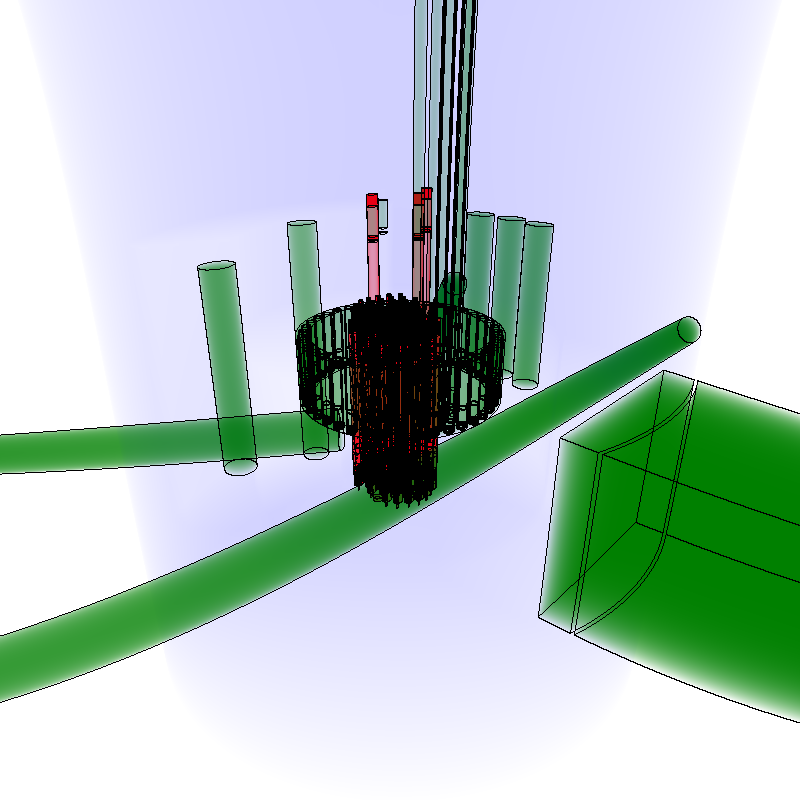
\includegraphics[width=\linewidth]{../images/triga.png}
    TRIGA reactor ex-core components.\\
    Model courtesy JSI, Slovenia.
  \end{columns}
\end{frame}

\begin{frame}{Surface meshes}
  \begin{itemize}
    \item Method of choice in computer graphics
    \item OpenMC can use surface meshes via DAGMC
    \item We could, for example, calculate the $k$ eigenvalue
      of my friend Lorenzo if he were made of plutonium
  \end{itemize}
  \begin{columns}
    \column{0.45\textwidth}
    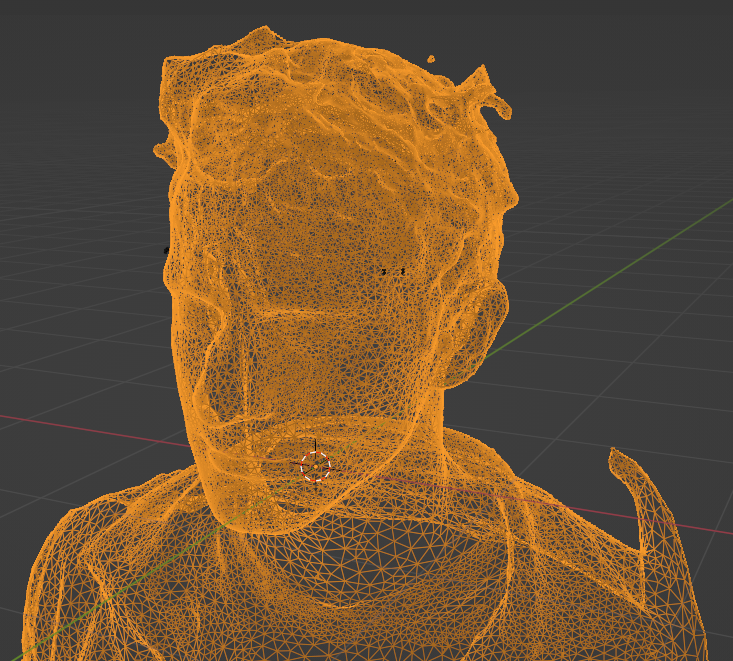
\includegraphics[width=\linewidth]{../images/lorenzo_head.png}
    Lorenzo's head triangulation
    \column{0.45\textwidth}
    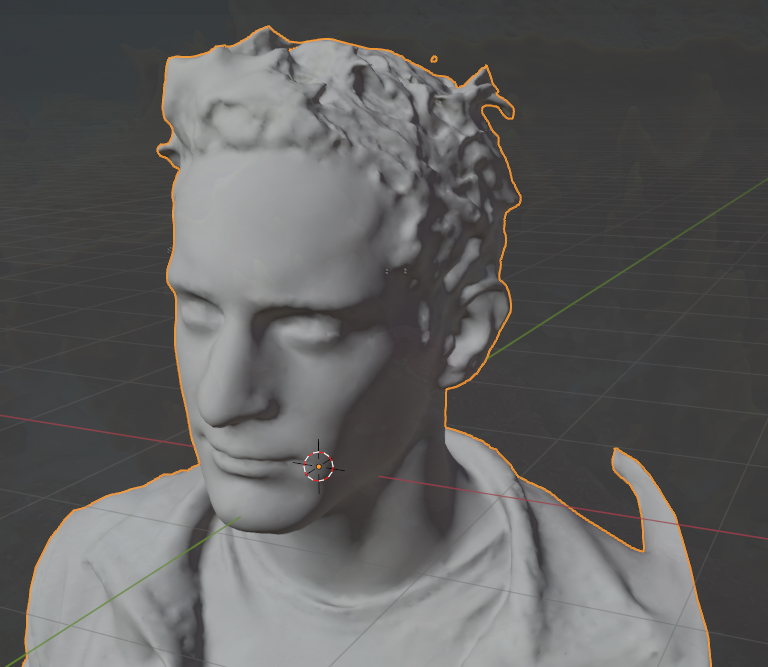
\includegraphics[width=\linewidth]{../images/lorenzo_head_solid.png}
    resulting surface
  \end{columns}
\end{frame}

\begin{frame}{Volume meshes}
  \begin{columns}
    \column{0.45\textwidth}
    \begin{itemize}
      \item Commonly used to calculate stresses in parts, heat transfer, CFD, etc.
      \item OpenMC \textbf{cannot} natively define problem geometries using volume meshes,
        but tallying \textbf{can} be done on volume meshes
      \item Tools associated with DAGMC can be used to extract surface meshes from
        volume meshes for use with OpenMC
      \item More info: \url{svalinn.github.io/DAGMC/usersguide/}
    \end{itemize}
    \column{0.45\textwidth}
    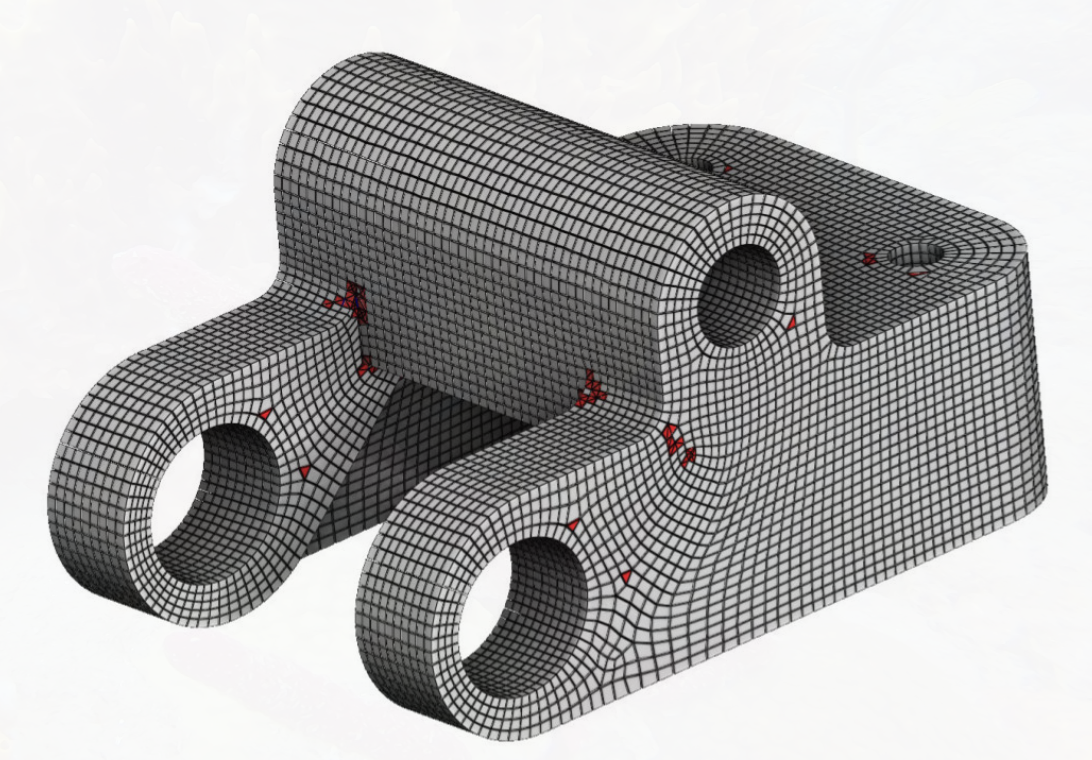
\includegraphics[width=\linewidth]{../images/hexmesh.png}
    For example, hex meshes are lots of little deformed bricks put together
  \end{columns}
  \footnotetext{Image: \textit{Hexahedral Meshing: Mind the Gap!}. Ray, Sokolov, et. al. \url{hal.inria.fr/hal-01551603/document}}
\end{frame}

\begin{frame}{Voxelization}
  \begin{columns}
    \column{0.45\textwidth}
    \begin{itemize}
      \item Many radiation simulating programs employ voxelization
      \item Los Alamos Nat'l Lab's PARTISN
      \item numerous health physics codes
      \item \textbf{OpenMC does not rely on or use voxelization}
    \end{itemize}
    \column{0.45\textwidth}
    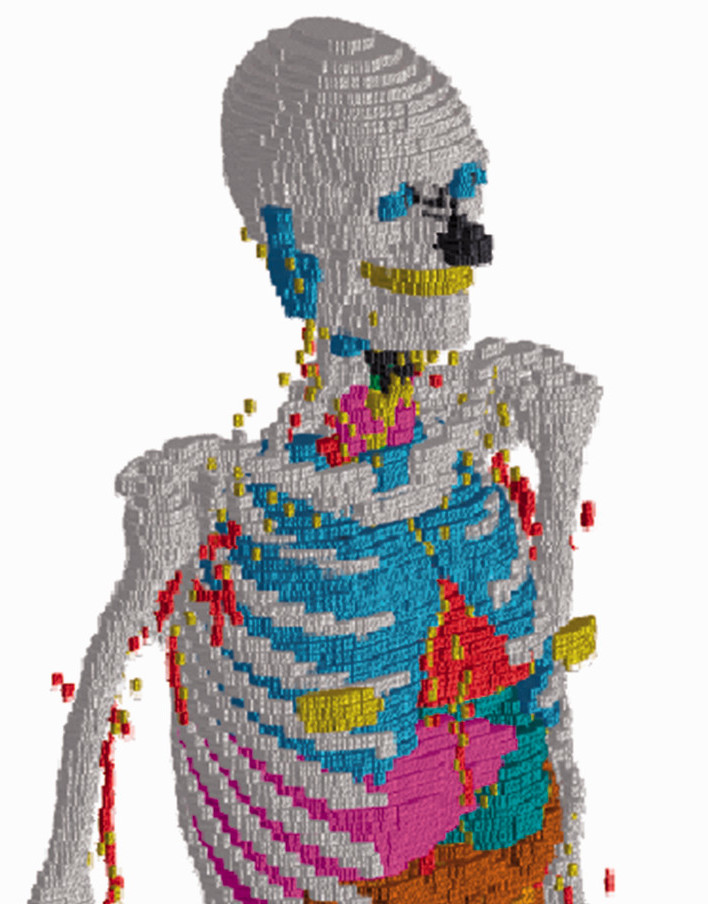
\includegraphics[width=0.7\linewidth]{../images/medical_phantom.jpeg}\\
    Medical phantom
  \end{columns}
  \footnotetext{Image: \textit{Computational phantoms, ICRP/ICRU, and further developments}. Zankl, Becker et. al. Annals of the ICRP, 2018.}
\end{frame}

\begin{frame}{Computational Solid Geometry}
  \begin{itemize}
    \item Let's start from the absolute basics!
    \item Suppose we want to solve a 2D problem like this one:
    \item How to define using OpenMC's CSG?
  \end{itemize}
\end{frame}

\begin{frame}{Computational Solid Geometry}
  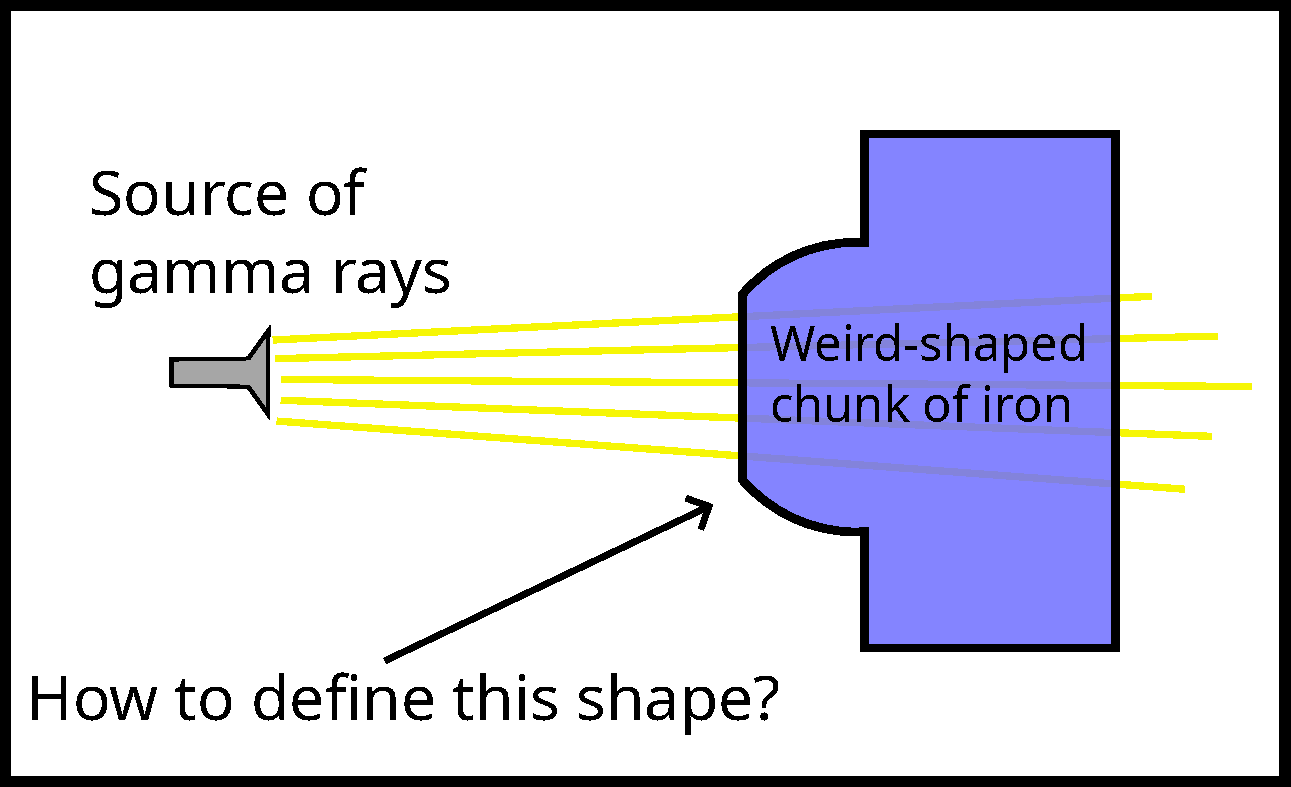
\includegraphics[width=\textwidth]{../images/csg1.pdf}
\end{frame}
\begin{frame}{Computational Solid Geometry}
  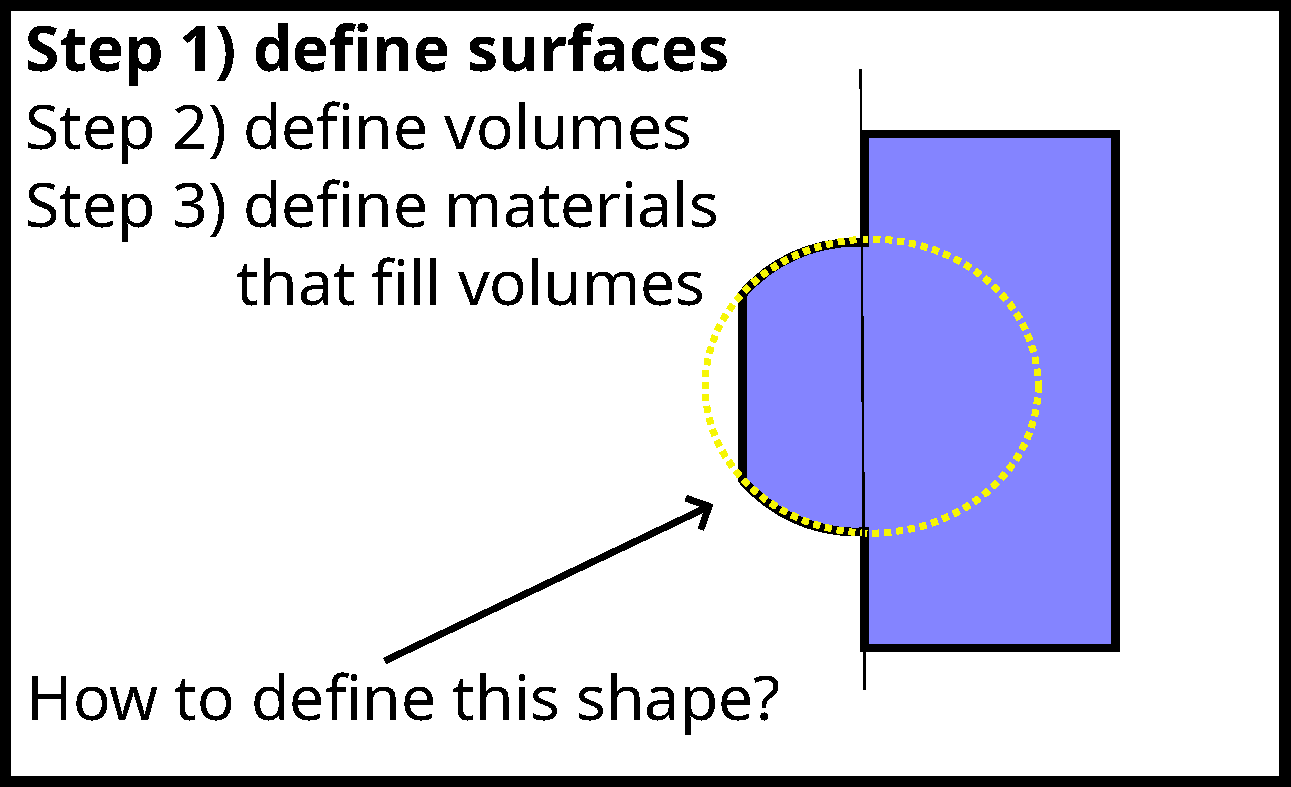
\includegraphics[width=\textwidth]{../images/csg2.pdf}
\end{frame}
\begin{frame}{Computational Solid Geometry}
  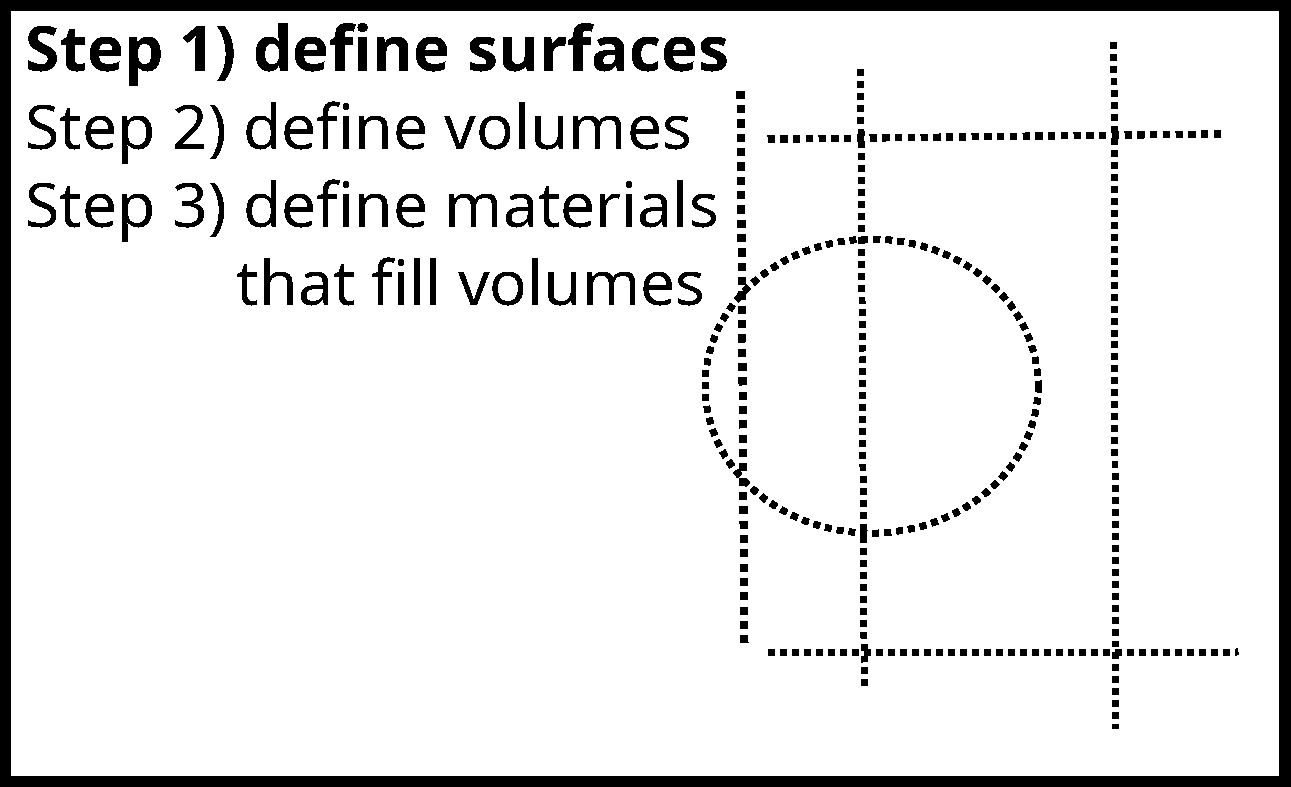
\includegraphics[width=\textwidth]{../images/csg3.pdf}
\end{frame}
\begin{frame}{Computational Solid Geometry}
  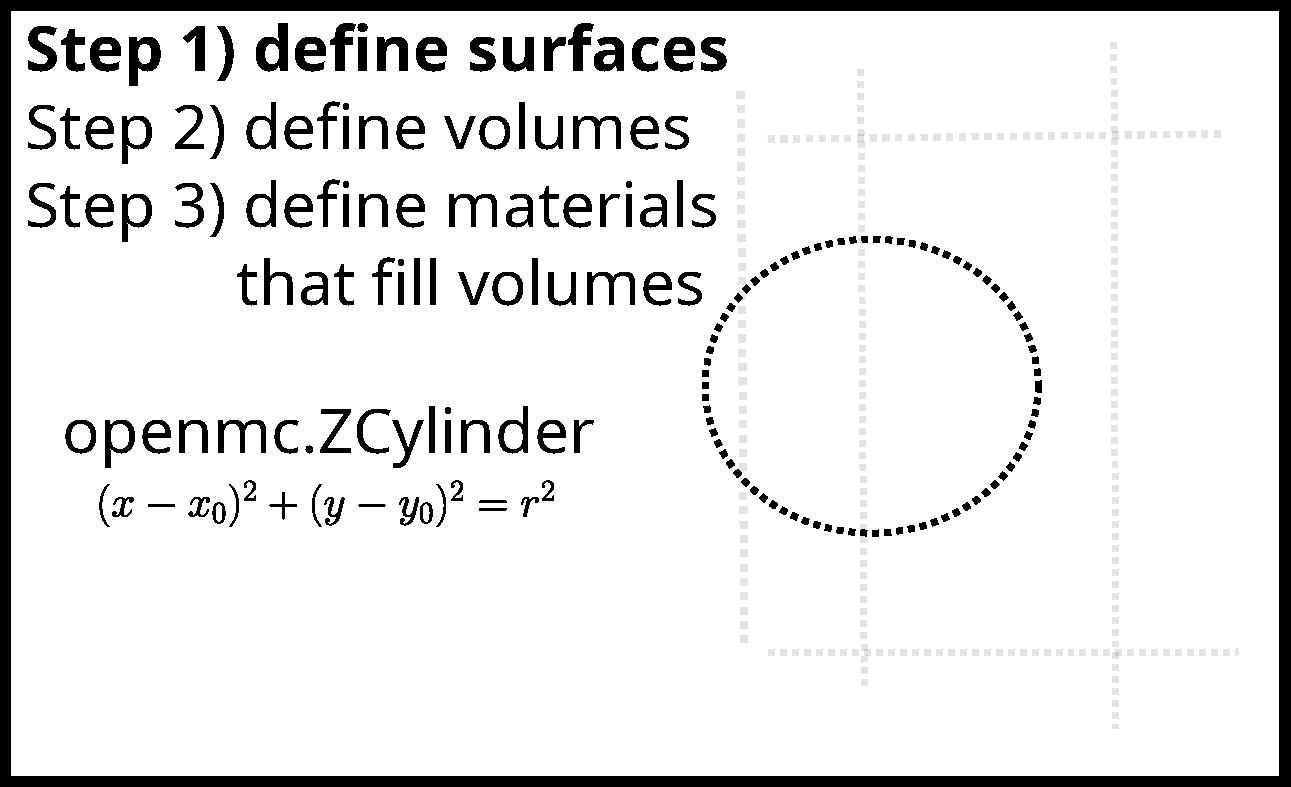
\includegraphics[width=\textwidth]{../images/csg4.pdf}
\end{frame}
\begin{frame}{Computational Solid Geometry}
  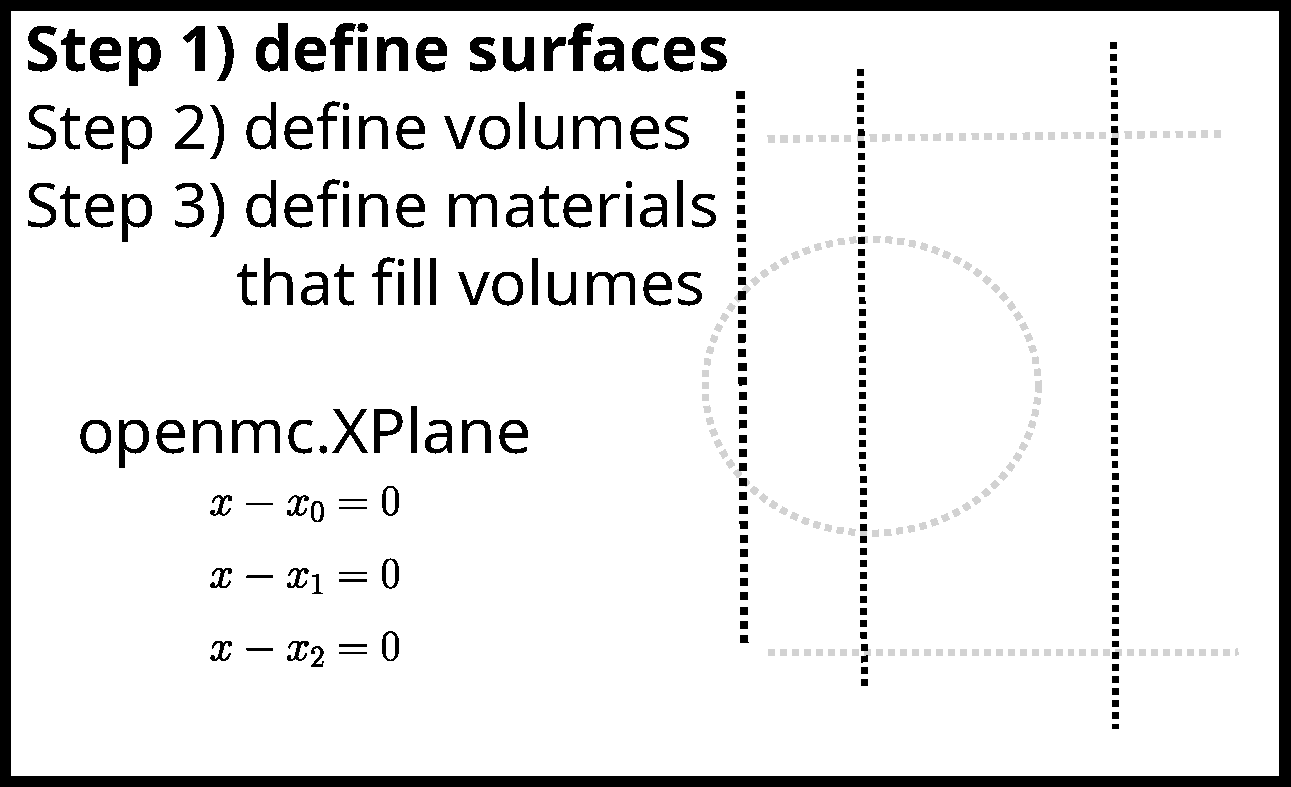
\includegraphics[width=\textwidth]{../images/csg5.pdf}
\end{frame}
\begin{frame}{Computational Solid Geometry}
  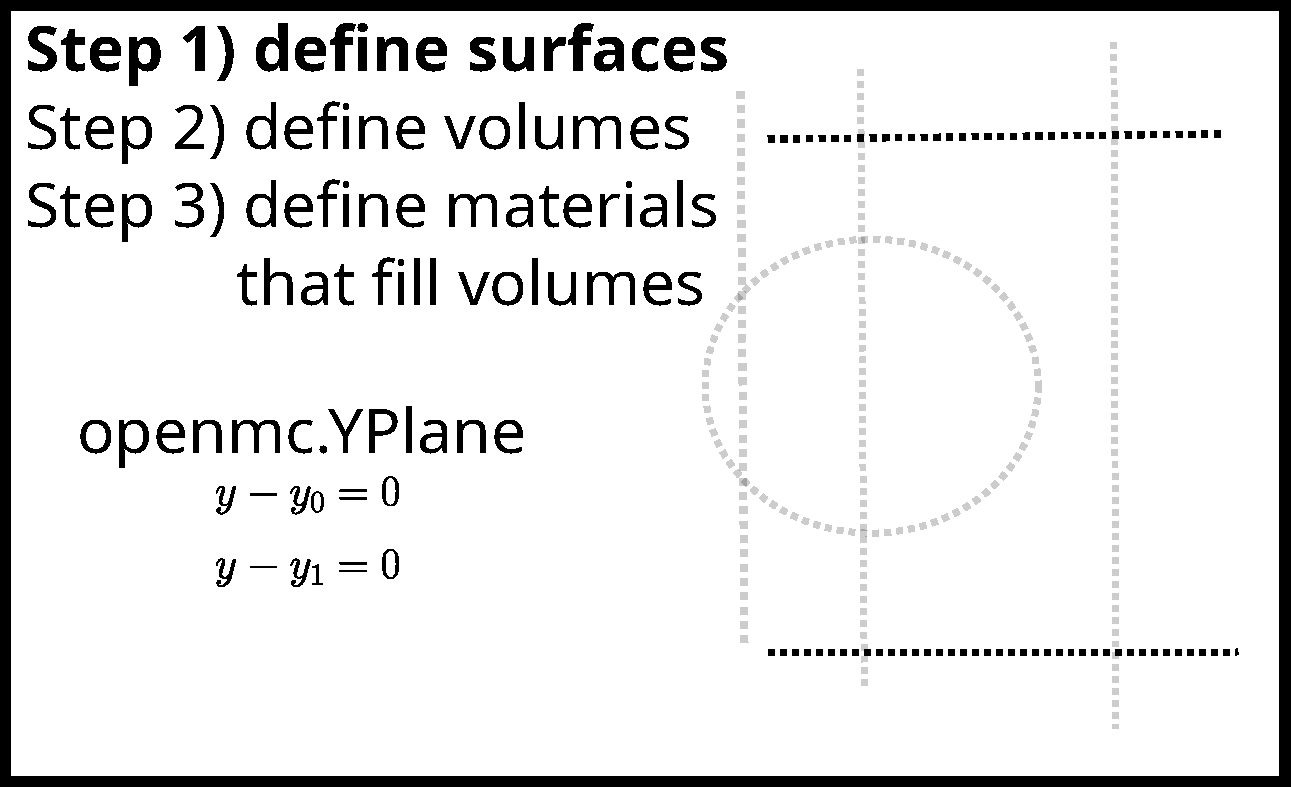
\includegraphics[width=\textwidth]{../images/csg6.pdf}
\end{frame}
\begin{frame}{Computational Solid Geometry}
  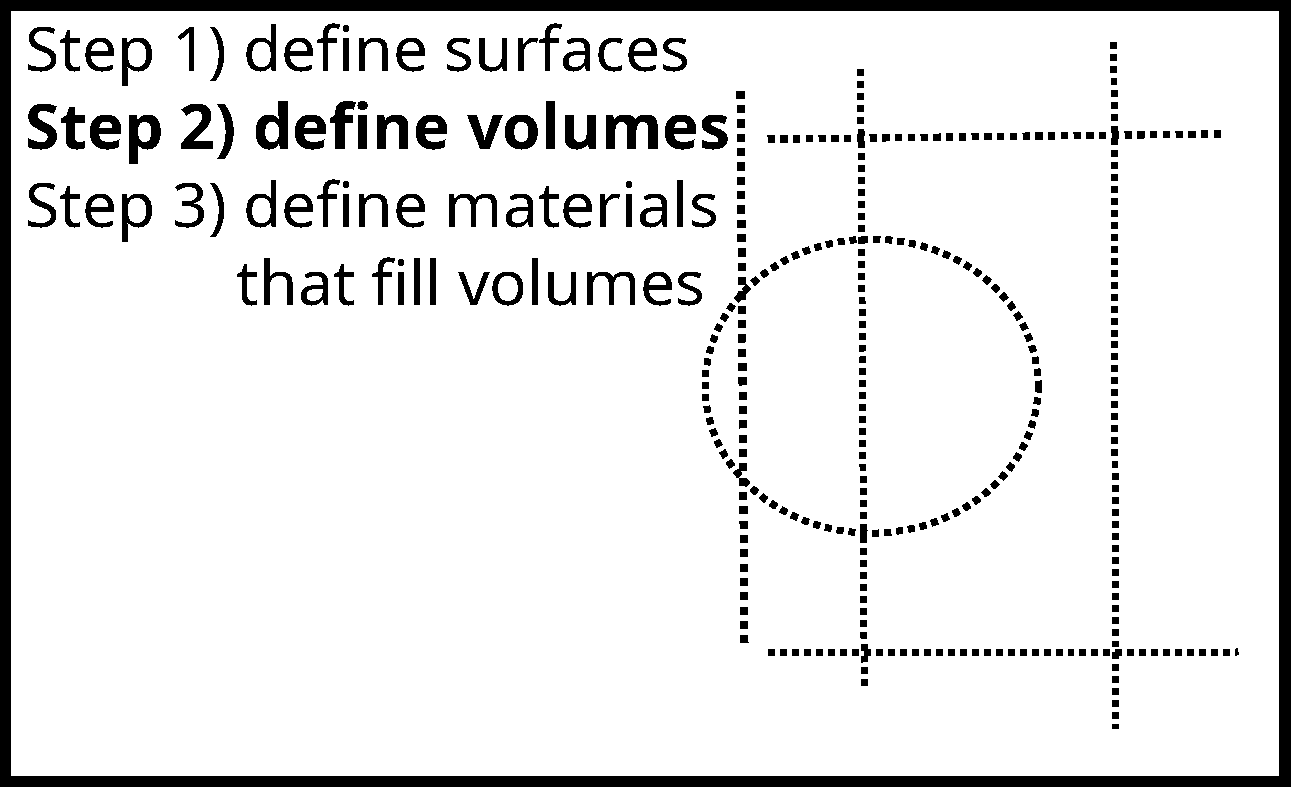
\includegraphics[width=\textwidth]{../images/csg7.pdf}
\end{frame}
\begin{frame}{Computational Solid Geometry}
  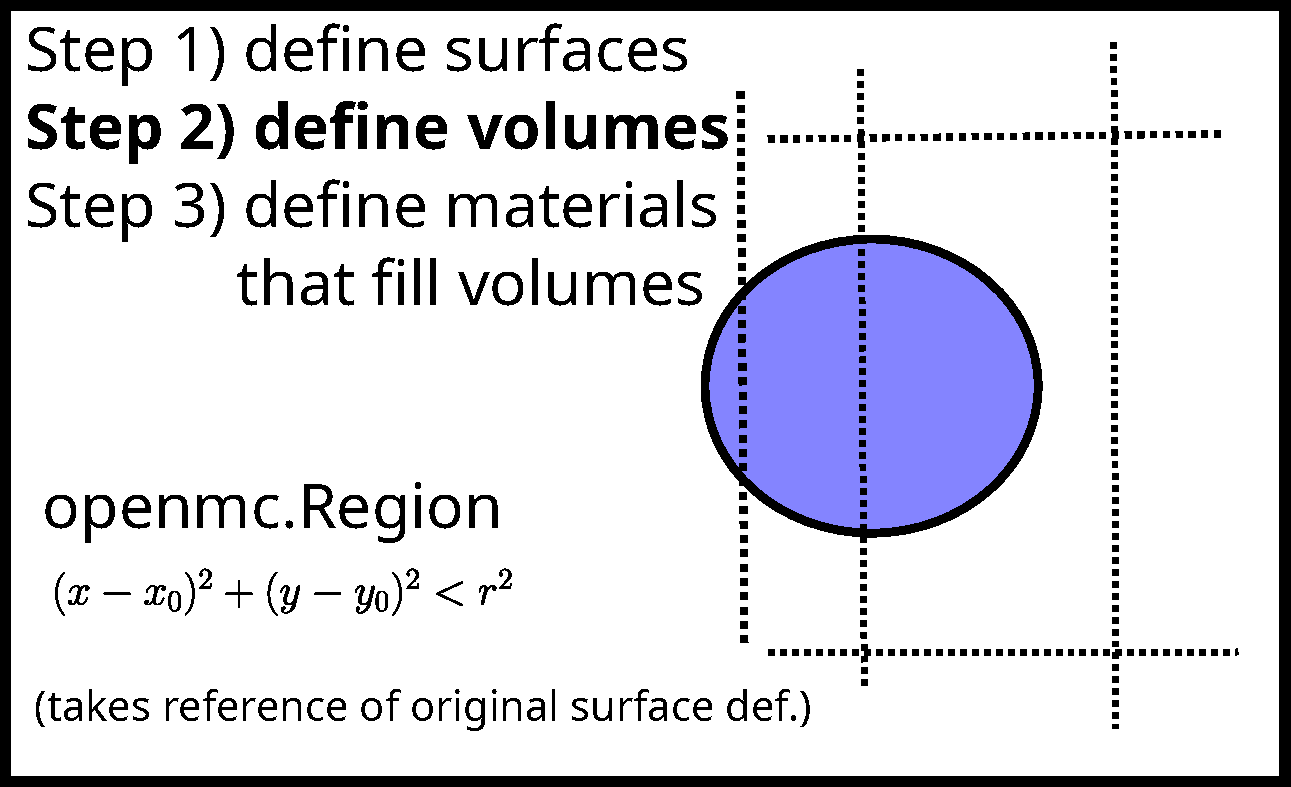
\includegraphics[width=\textwidth]{../images/csg8.pdf}
\end{frame}
\begin{frame}{Computational Solid Geometry}
  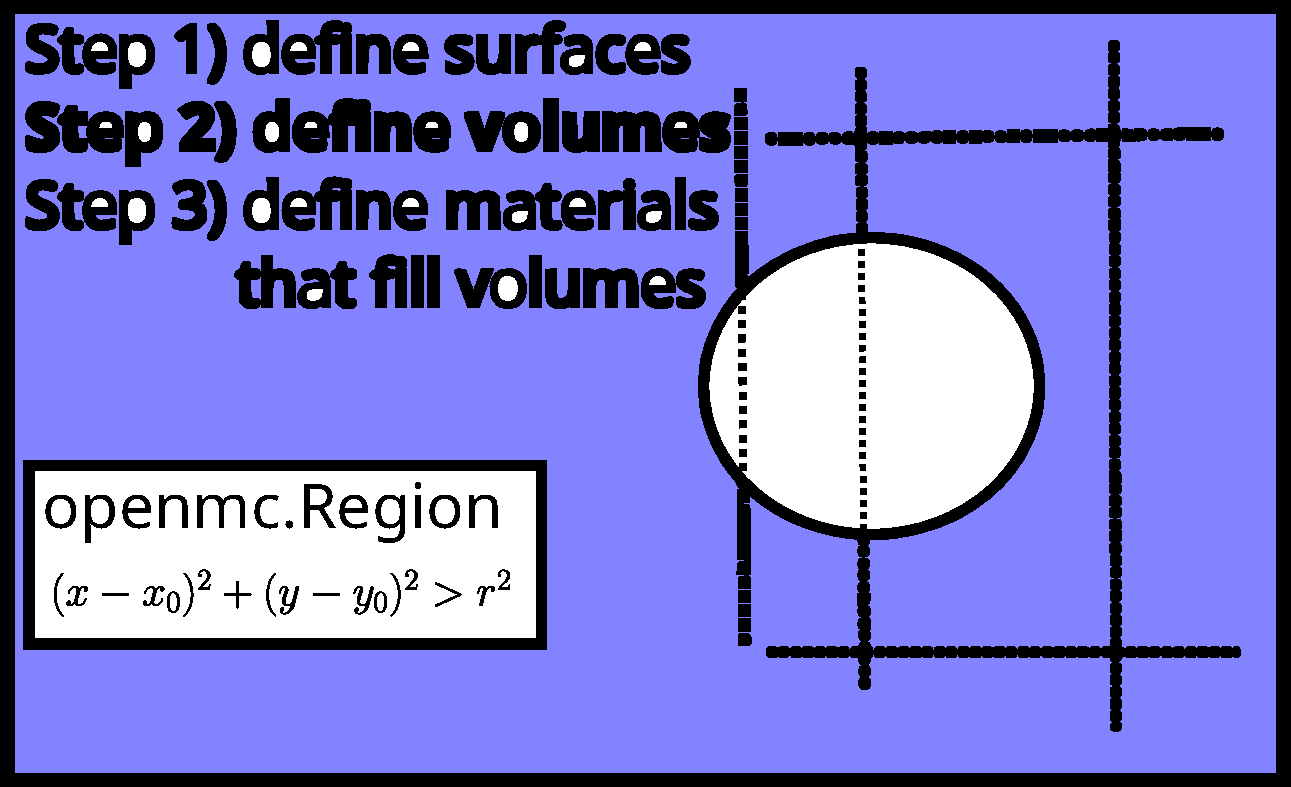
\includegraphics[width=\textwidth]{../images/csg9.pdf}
\end{frame}
\begin{frame}{Computational Solid Geometry}
  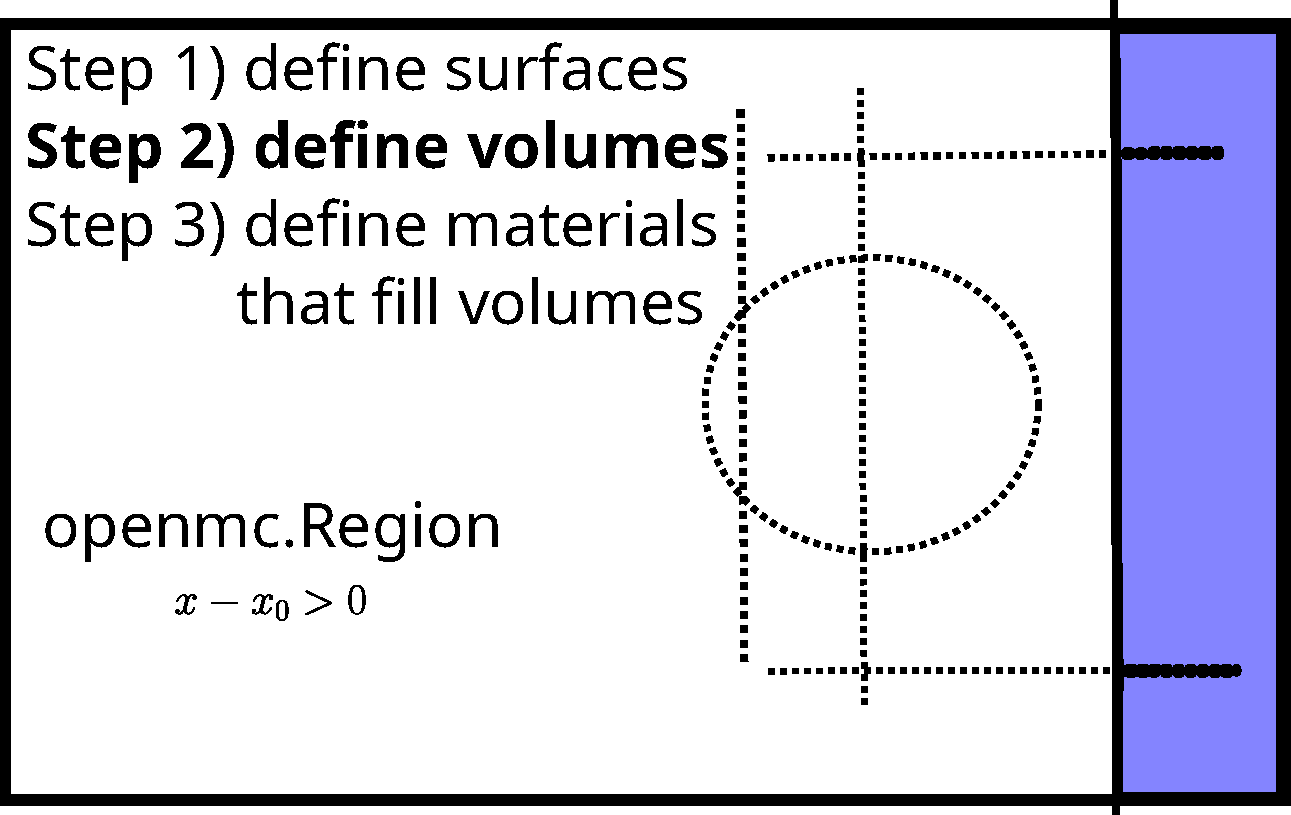
\includegraphics[width=\textwidth]{../images/csg10.pdf}
\end{frame}
\begin{frame}{Computational Solid Geometry}
  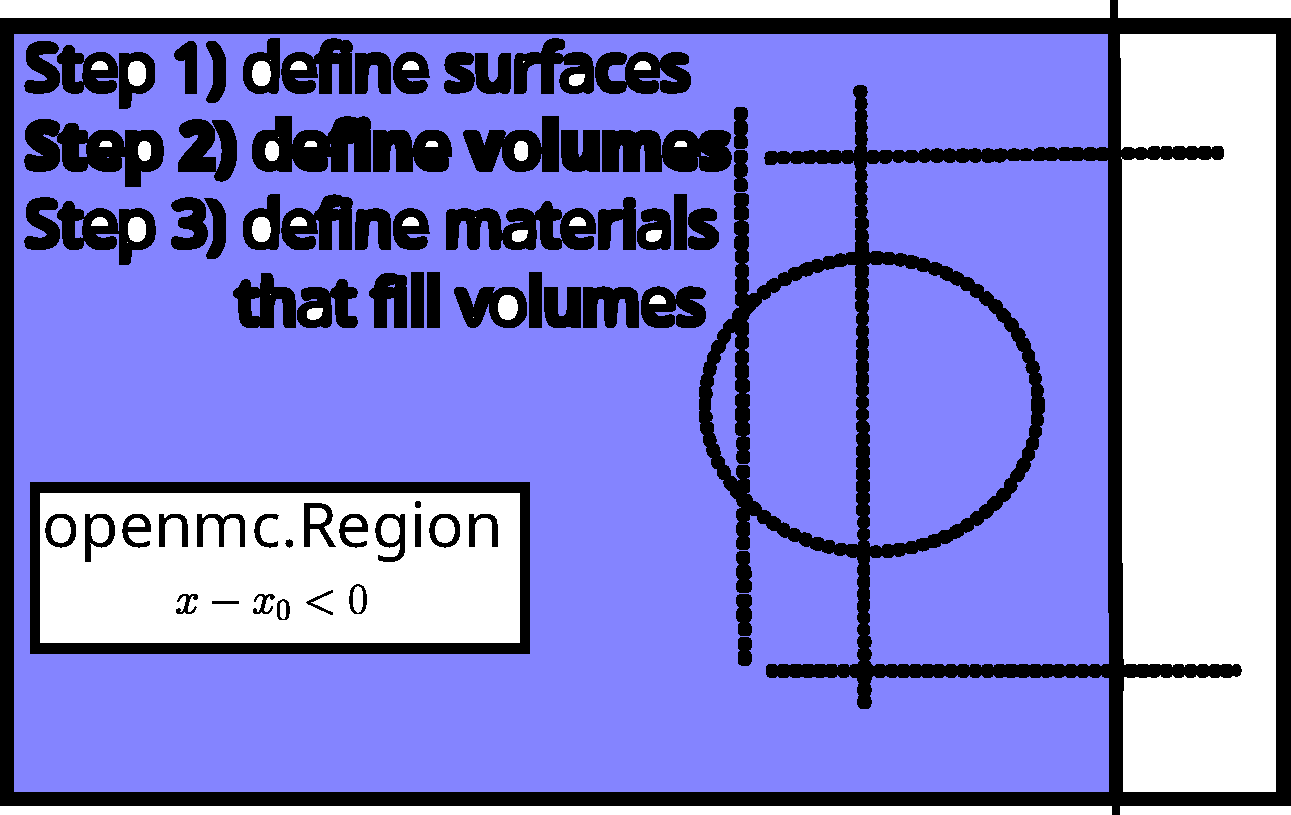
\includegraphics[width=\textwidth]{../images/csg11.pdf}
\end{frame}
\begin{frame}{Computational Solid Geometry}
  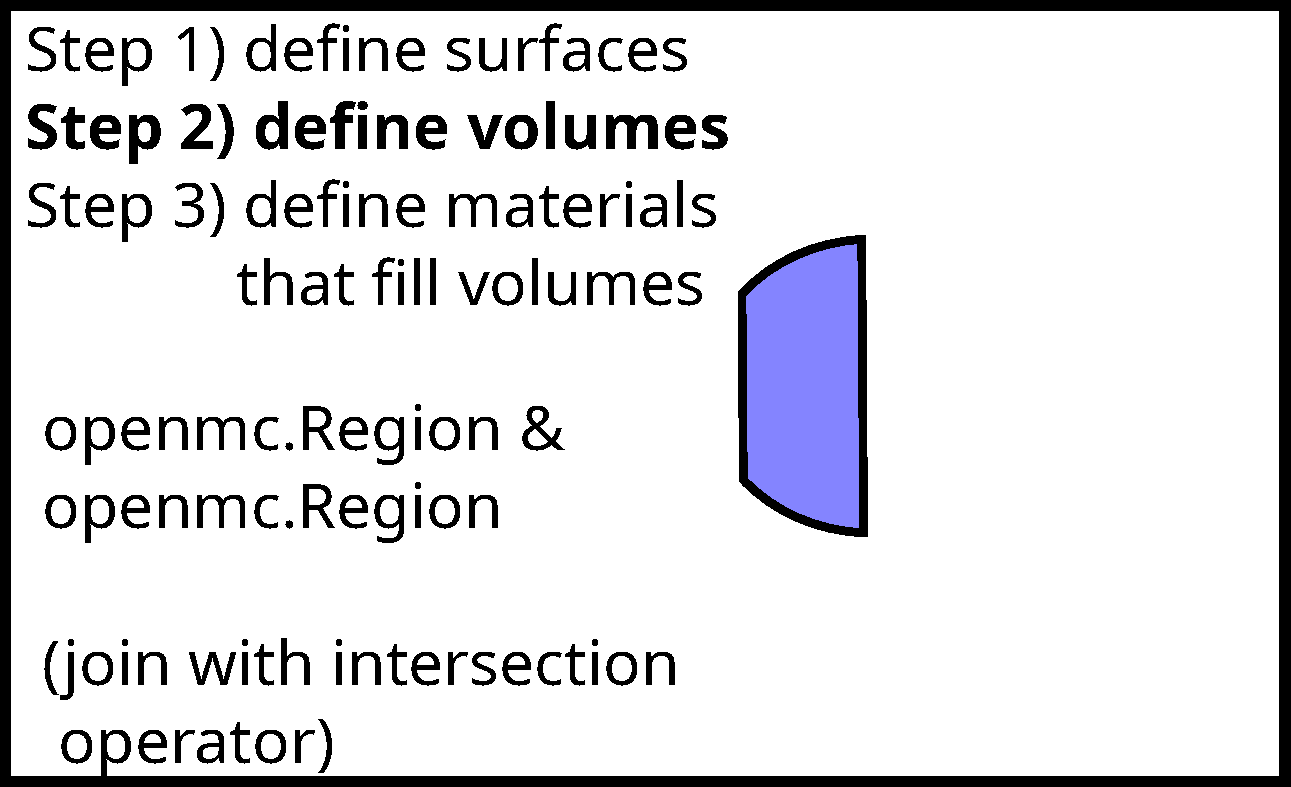
\includegraphics[width=\textwidth]{../images/csg12.pdf}
\end{frame}
\begin{frame}{Computational Solid Geometry}
  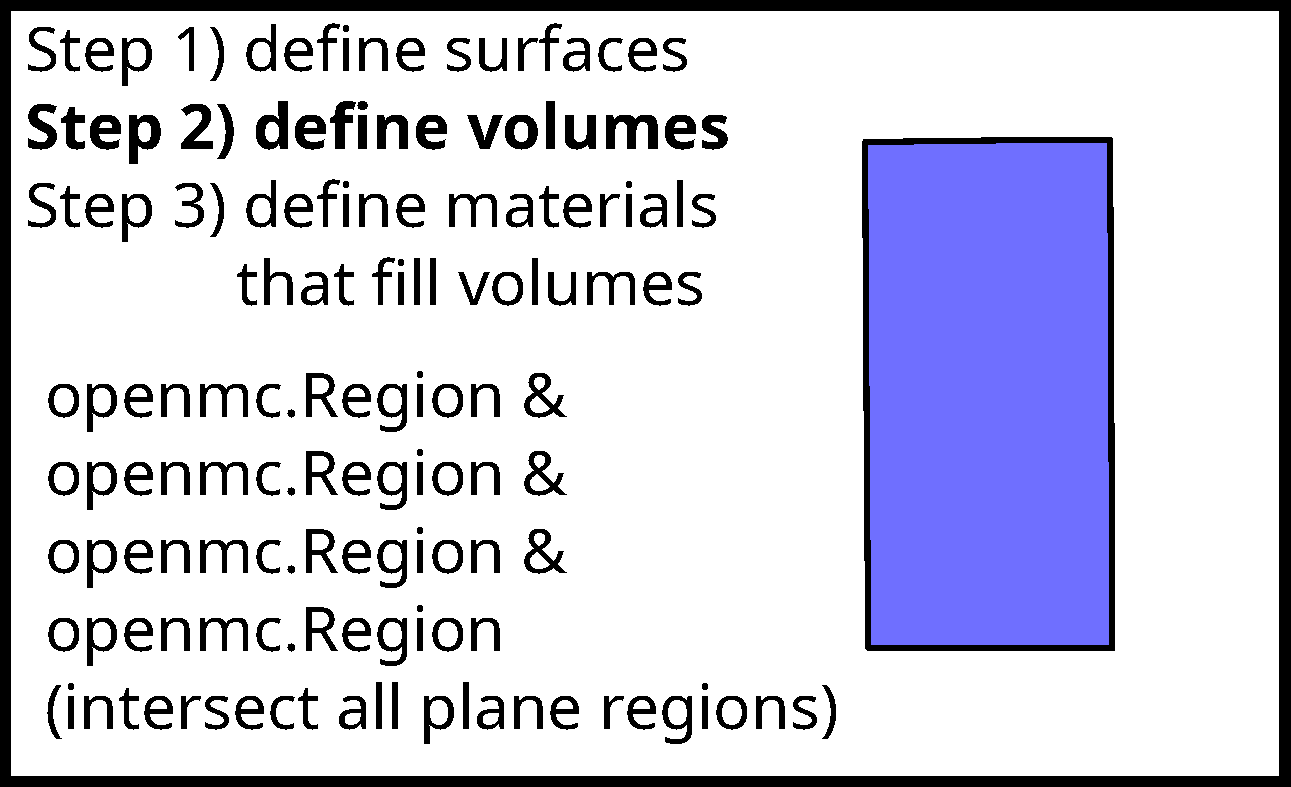
\includegraphics[width=\textwidth]{../images/csg13.pdf}
\end{frame}
\begin{frame}{Computational Solid Geometry}
  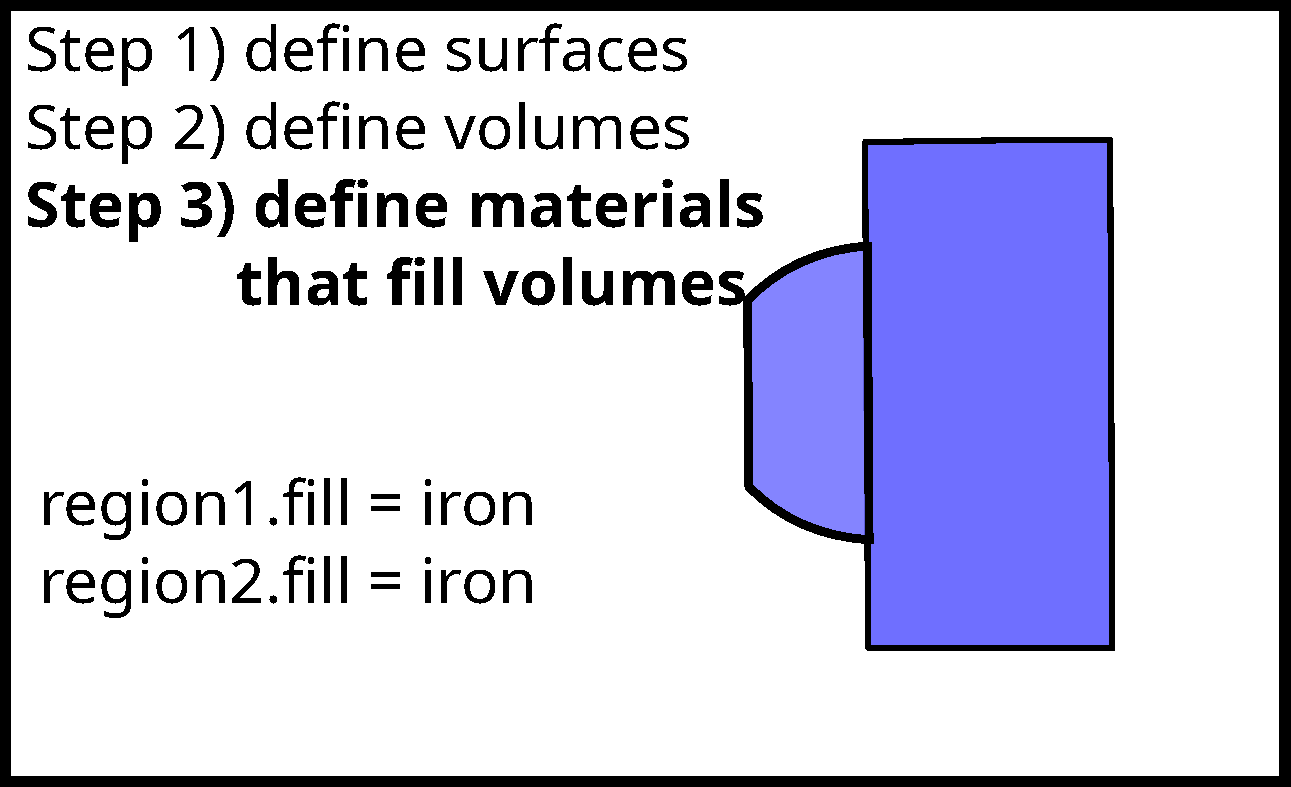
\includegraphics[width=\textwidth]{../images/csg14.pdf}
\end{frame}

%%---------------------------------------------------------------------------%%

\end{document}
